\documentclass[11pt,oneside]{article}

\pdfminorversion=7
\usepackage{QuizStyle}
\usepackage{tikz}
\usetikzlibrary{arrows.meta,calc,decorations.markings,positioning}
\tikzset{
  quizvertex/.style={circle,fill=black,inner sep=1.9pt},
  quizedge/.style={line width=0.58pt},
  quizarc/.style={-{Stealth[length=2.15mm,width=1.45mm]},line width=0.61pt,shorten <=3pt,shorten >=3pt},
  quizmultiarc/.style={line width=0.55pt,postaction={decorate},decoration={markings,mark=at position 0.53 with {\arrow{Stealth[length=1.75mm,width=1.20mm]}}}},
  quizloop/.style={line width=0.61pt,postaction={decorate},decoration={markings,mark=at position 0.62 with {\arrow{Stealth[length=2.15mm,width=1.45mm]}}}}
}
\hypersetup{
  pdftitle={20261112 Quiz for MATH261 Discrete Mathematics},
  pdfauthor={Jungwoo Kim},
  pdfsubject={Homework 4 problems and solutions for MATH261 Discrete Mathematics},
  pdfcreator={LaTeX}
}

\begin{document}
\quiztitle{20261112 Quiz}

\begin{problem}{1}
\begin{problemsubparts}
\item Draw the directed graph represented by the given adjacency matrix.
\item Find the adjacency matrix of the given directed multigraph.
\end{problemsubparts}
\begin{center}
\begin{minipage}[c]{0.38\textwidth}\centering
\[
\mathbf A=\begin{pmatrix}
0&1&3&0&4\\
1&2&1&3&0\\
3&1&1&0&1\\
0&3&0&0&2\\
4&0&1&2&3
\end{pmatrix}.
\]
\end{minipage}\hfill
\begin{minipage}[c]{0.54\textwidth}\centering
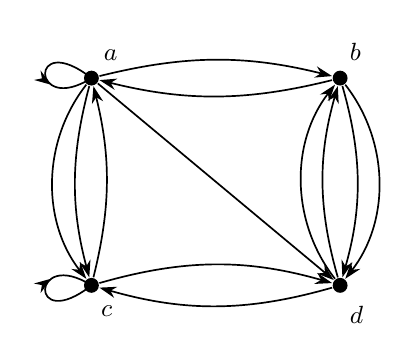
\begin{tikzpicture}[x=1cm,y=1cm,scale=0.94]
\coordinate (a) at (-1.68,1.40);
\coordinate (b) at (1.68,1.40);
\coordinate (c) at (-1.68,-1.40);
\coordinate (d) at (1.68,-1.40);
% Opposite arrows and parallel arcs are separated into distinct lanes.
\draw[quizarc] (a) to[bend left=14] (b);
\draw[quizarc] (b) to[bend left=14] (a);
\draw[quizarc] (a) to[bend right=15] (c);
\draw[quizarc] (a) to[bend right=38] (c);
\draw[quizarc] (c) to[bend right=14] (a);
\draw[quizarc] (a) -- (d);
\draw[quizarc] (b) to[bend left=16] (d);
\draw[quizarc] (b) to[bend left=38] (d);
\draw[quizarc] (d) to[bend left=16] (b);
\draw[quizarc] (d) to[bend left=38] (b);
\draw[quizarc] (c) to[bend left=16] (d);
\draw[quizarc] (d) to[bend left=16] (c);
% Put arrowheads on the loops themselves, not beneath a vertex dot.
\draw[quizloop] (a) .. controls +(-0.85,0.67) and +(-0.82,-0.52) .. (a);
\draw[quizloop] (c) .. controls +(-0.85,-0.67) and +(-0.82,0.52) .. (c);
\foreach \v in {a,b,c,d}{\node[quizvertex] at (\v) {};}
\node[font=\small,above right=3pt and 1pt] at (a) {$a$};
\node[font=\small,above right=3pt and 0pt] at (b) {$b$};
\node[font=\small,below right=4pt and 0pt] at (c) {$c$};
\node[font=\small,below right=4pt and 0pt] at (d) {$d$};
\end{tikzpicture}
\end{minipage}
\end{center}
\end{problem}

\begin{solution}
\begin{problemsubparts}
\item Drawing each arc separately, including the loops, gives the following
 directed multigraph.
\begin{center}
% Each drawn curve is one directed arc. Arrowheads are at mid-curve to avoid crowded vertices.
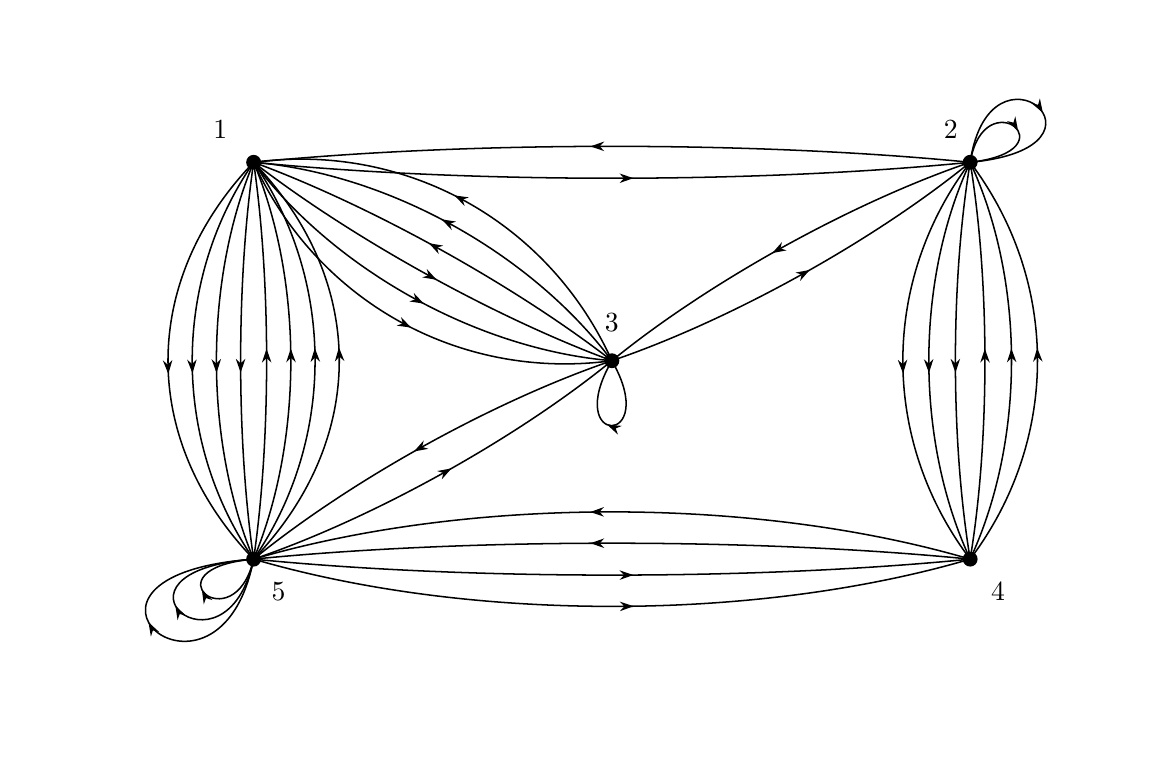
\begin{tikzpicture}[x=1cm,y=1cm]
\coordinate (v1) at (-4.55,2.52);
\coordinate (v2) at (4.55,2.52);
\coordinate (v3) at (0,0);
\coordinate (v4) at (4.55,-2.52);
\coordinate (v5) at (-4.55,-2.52);
% Non-loop arcs: 30 total.
\draw[quizmultiarc] (v1) .. controls (-1.820,2.250) and (1.820,2.250) .. (v2);
\draw[quizmultiarc] (v2) .. controls (1.820,2.790) and (-1.820,2.790) .. (v1);

\draw[quizmultiarc] (v1) .. controls (-3.747,0.749) and (-1.927,-0.259) .. (v3);
\draw[quizmultiarc] (v1) .. controls (-3.524,1.152) and (-1.704,0.144) .. (v3);
\draw[quizmultiarc] (v1) .. controls (-3.301,1.554) and (-1.481,0.546) .. (v3);
\draw[quizmultiarc] (v3) .. controls (-1.249,0.966) and (-3.069,1.974) .. (v1);
\draw[quizmultiarc] (v3) .. controls (-1.026,1.368) and (-2.846,2.376) .. (v1);
\draw[quizmultiarc] (v3) .. controls (-0.803,1.771) and (-2.623,2.779) .. (v1);

\draw[quizmultiarc] (v1) .. controls (-6.000,1.008) and (-6.000,-1.008) .. (v5);
\draw[quizmultiarc] (v1) .. controls (-5.590,1.008) and (-5.590,-1.008) .. (v5);
\draw[quizmultiarc] (v1) .. controls (-5.180,1.008) and (-5.180,-1.008) .. (v5);
\draw[quizmultiarc] (v1) .. controls (-4.770,1.008) and (-4.770,-1.008) .. (v5);
\draw[quizmultiarc] (v5) .. controls (-4.330,-1.008) and (-4.330,1.008) .. (v1);
\draw[quizmultiarc] (v5) .. controls (-3.920,-1.008) and (-3.920,1.008) .. (v1);
\draw[quizmultiarc] (v5) .. controls (-3.510,-1.008) and (-3.510,1.008) .. (v1);
\draw[quizmultiarc] (v5) .. controls (-3.100,-1.008) and (-3.100,1.008) .. (v1);

\draw[quizmultiarc] (v2) .. controls (3.049,2.009) and (1.229,1.001) .. (v3);
\draw[quizmultiarc] (v3) .. controls (1.501,0.511) and (3.321,1.519) .. (v2);

\draw[quizmultiarc] (v2) .. controls (3.410,1.008) and (3.410,-1.008) .. (v4);
\draw[quizmultiarc] (v2) .. controls (3.850,1.008) and (3.850,-1.008) .. (v4);
\draw[quizmultiarc] (v2) .. controls (4.300,1.008) and (4.300,-1.008) .. (v4);
\draw[quizmultiarc] (v4) .. controls (4.800,-1.008) and (4.800,1.008) .. (v2);
\draw[quizmultiarc] (v4) .. controls (5.250,-1.008) and (5.250,1.008) .. (v2);
\draw[quizmultiarc] (v4) .. controls (5.690,-1.008) and (5.690,1.008) .. (v2);

\draw[quizmultiarc] (v3) .. controls (-1.501,-0.511) and (-3.321,-1.519) .. (v5);
\draw[quizmultiarc] (v5) .. controls (-3.049,-2.009) and (-1.229,-1.001) .. (v3);

\draw[quizmultiarc] (v4) .. controls (1.820,-1.720) and (-1.820,-1.720) .. (v5);
\draw[quizmultiarc] (v4) .. controls (1.820,-2.250) and (-1.820,-2.250) .. (v5);
\draw[quizmultiarc] (v5) .. controls (-1.820,-2.790) and (1.820,-2.790) .. (v4);
\draw[quizmultiarc] (v5) .. controls (-1.820,-3.320) and (1.820,-3.320) .. (v4);

% Loops: two at 2, one at 3, three at 5.
\draw[quizmultiarc] (v2) .. controls (4.730,3.580) and (5.870,2.670) .. (v2);
\draw[quizmultiarc] (v2) .. controls (4.800,4.220) and (6.580,2.710) .. (v2);
\draw[quizmultiarc] (v3) .. controls (0.630,-1.100) and (-0.640,-1.100) .. (v3);
\draw[quizmultiarc] (v5) .. controls (-4.800,-3.590) and (-5.930,-2.640) .. (v5);
\draw[quizmultiarc] (v5) .. controls (-4.900,-4.170) and (-6.660,-2.680) .. (v5);
\draw[quizmultiarc] (v5) .. controls (-4.990,-4.760) and (-7.410,-2.730) .. (v5);
% Solid vertex dots mask arc endpoints.
\foreach \i in {1,2,3,4,5}{\node[quizvertex] at (v\i) {};}
\node[font=\normalsize,above left=5pt and 6pt] at (v1) {$1$};
\node[font=\normalsize,above left=5pt and 1pt] at (v2) {$2$};
\node[font=\normalsize,above=7pt] at (v3) {$3$};
\node[font=\normalsize,below right=5pt and 4pt] at (v4) {$4$};
\node[font=\normalsize,below right=5pt and 3pt] at (v5) {$5$};
\end{tikzpicture}
\end{center}
\item With rows and columns ordered as $a, b, c, d$, the adjacency matrix is
\[
\mathbf A=\begin{pmatrix}
1&1&2&1\\
1&0&0&2\\
1&0&1&1\\
0&2&1&0
\end{pmatrix}.
\]
\end{problemsubparts}
\end{solution}

\begin{problem}{2}
Consider the following directed graph.
\begin{problemsubparts}
\item Find all paths starting at vertex $a$ and ending at vertex $b$ or $c$.
Determine the length of each path.
\item Find all cycles starting at vertex $a$. Determine the length of each cycle.
\end{problemsubparts}
\begin{center}
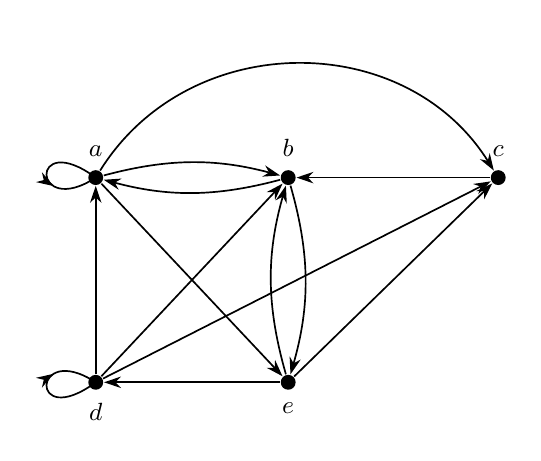
\begin{tikzpicture}[x=1cm,y=1cm,scale=0.97]
\coordinate (a) at (-2.52,1.34);
\coordinate (b) at (0,1.34);
\coordinate (c) at (2.75,1.34);
\coordinate (d) at (-2.52,-1.34);
\coordinate (e) at (0,-1.34);
\draw[quizarc] (a) to[bend left=15] (b);
\draw[quizarc] (b) to[bend left=15] (a);
\draw[quizarc] (a) to[out=58,in=122,looseness=1.12] (c);
\draw[quizarc] (a) -- (e);
\draw[quizarc] (b) to[bend left=16] (e);
\draw[quizarc] (e) to[bend left=16] (b);
\draw[quizarc] (c) -- (b);
\draw[quizarc] (d) -- (a);
\draw[quizarc] (d) -- (b);
\draw[quizarc] (d) -- (c);
\draw[quizarc] (e) -- (d);
\draw[quizarc] (e) -- (c);
\draw[quizloop] (a) .. controls +(-0.88,0.65) and +(-0.84,-0.55) .. (a);
\draw[quizloop] (d) .. controls +(-0.88,-0.65) and +(-0.84,0.55) .. (d);
\foreach \v in {a,b,c,d,e}{\node[quizvertex] at (\v) {};}
\node[font=\small,above=4pt] at (a) {$a$};
\node[font=\small,above=4pt] at (b) {$b$};
\node[font=\small,above=4pt] at (c) {$c$};
\node[font=\small,below=4pt] at (d) {$d$};
\node[font=\small,below=4pt] at (e) {$e$};
\end{tikzpicture}
\end{center}
\end{problem}

\begin{solution}
\begin{problemsubparts}
\item A path cannot repeat a vertex. The paths are listed below, grouped
by their terminal vertices; the number in parentheses is the length.
\[
\begin{array}{l@{\qquad}l}
\text{Ending at }b & \text{Ending at }c \\[2pt]
(a,b)\ (1) &(a,c)\ (1)\\
(a,c,b)\ (2) &(a,e,c)\ (2)\\
(a,e,b)\ (2) &(a,b,e,c)\ (3)\\
(a,e,c,b)\ (3) &(a,e,d,c)\ (3)\\
(a,e,d,b)\ (3) &(a,b,e,d,c)\ (4)\\
(a,e,d,c,b)\ (4) &
\end{array}
\]
These $11$ paths are exhaustive: the first edge from $a$ goes to $b$,
$c$, or $e$, and no vertex may be revisited.

\item A cycle returns to its initial vertex without repeating any other vertex.
The cycles starting at $a$, grouped by length, are
\[
\begin{array}{c@{\qquad}l}
\text{Length}&\text{Cycle}\\ \hline
1&(a,a)\\
2&(a,b,a)\\
3&(a,c,b,a),\ (a,e,b,a),\ (a,e,d,a)\\
4&(a,b,e,d,a),\ (a,e,c,b,a),\ (a,e,d,b,a)\\
5&(a,c,b,e,d,a),\ (a,e,d,c,b,a)
\end{array}
\]
There are $10$ cycles in total, including the loop $(a,a)$ and the directed
$2$-cycle $(a,b,a)$ under the course definition. Checking the first edge
from $a$ and forbidding repeated intermediate vertices proves exhaustiveness.
\end{problemsubparts}
\end{solution}

\begin{problem}{3}
Show that isomorphism of simple graphs is an equivalence relation.
\end{problem}
\begin{solution}
For every simple graph $G$, the identity on $V(G)$ is an isomorphism,
so the relation is reflexive. If $f\colon V(G)\to V(H)$ is an isomorphism,
then $f^{-1}\colon V(H)\to V(G)$ is also one, proving symmetry. Finally,
if $f\colon V(G)\to V(H)$ and $g\colon V(H)\to V(K)$ are isomorphisms,
so is $g\circ f$, proving transitivity. Thus graph isomorphism is an
equivalence relation.
\end{solution}

\begin{problem}{4}
Determine whether the given pair of graphs is isomorphic. Exhibit an
isomorphism or provide a rigorous argument that none exists.
\begin{center}
\begin{minipage}{0.48\textwidth}\centering
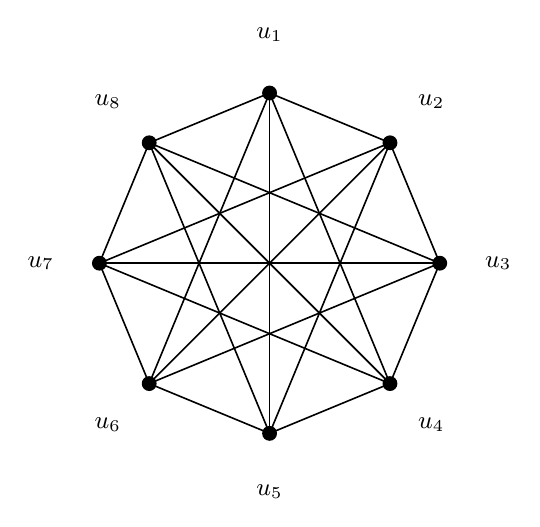
\begin{tikzpicture}[x=1cm,y=1cm,scale=1.46]
\coordinate (u0) at (0.000,1.480);
\node[font=\small,inner sep=0pt] at (0.000,1.990) {$u_{1}$};
\coordinate (u1) at (1.047,1.047);
\node[font=\small,inner sep=0pt] at (1.407,1.407) {$u_{2}$};
\coordinate (u2) at (1.480,0.000);
\node[font=\small,inner sep=0pt] at (1.990,0.000) {$u_{3}$};
\coordinate (u3) at (1.047,-1.047);
\node[font=\small,inner sep=0pt] at (1.407,-1.407) {$u_{4}$};
\coordinate (u4) at (0.000,-1.480);
\node[font=\small,inner sep=0pt] at (0.000,-1.990) {$u_{5}$};
\coordinate (u5) at (-1.047,-1.047);
\node[font=\small,inner sep=0pt] at (-1.407,-1.407) {$u_{6}$};
\coordinate (u6) at (-1.480,-0.000);
\node[font=\small,inner sep=0pt] at (-1.990,-0.000) {$u_{7}$};
\coordinate (u7) at (-1.047,1.047);
\node[font=\small,inner sep=0pt] at (-1.407,1.407) {$u_{8}$};
\draw[quizedge] (u0) -- (u1);
\draw[quizedge] (u0) -- (u3);
\draw[quizedge] (u0) -- (u4);
\draw[quizedge] (u0) -- (u5);
\draw[quizedge] (u0) -- (u7);
\draw[quizedge] (u1) -- (u2);
\draw[quizedge] (u1) -- (u4);
\draw[quizedge] (u1) -- (u5);
\draw[quizedge] (u1) -- (u6);
\draw[quizedge] (u2) -- (u3);
\draw[quizedge] (u2) -- (u5);
\draw[quizedge] (u2) -- (u6);
\draw[quizedge] (u2) -- (u7);
\draw[quizedge] (u3) -- (u4);
\draw[quizedge] (u3) -- (u6);
\draw[quizedge] (u3) -- (u7);
\draw[quizedge] (u4) -- (u5);
\draw[quizedge] (u4) -- (u7);
\draw[quizedge] (u5) -- (u6);
\draw[quizedge] (u6) -- (u7);
\node[quizvertex] at (u0) {};
\node[quizvertex] at (u1) {};
\node[quizvertex] at (u2) {};
\node[quizvertex] at (u3) {};
\node[quizvertex] at (u4) {};
\node[quizvertex] at (u5) {};
\node[quizvertex] at (u6) {};
\node[quizvertex] at (u7) {};
\end{tikzpicture}
\end{minipage}\hfill
\begin{minipage}{0.48\textwidth}\centering
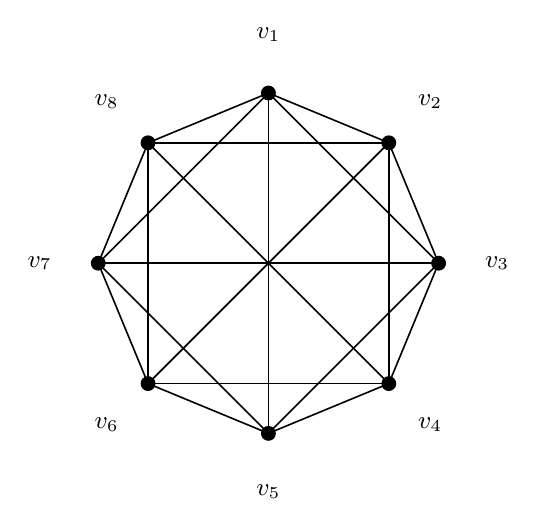
\begin{tikzpicture}[x=1cm,y=1cm,scale=1.46]
\coordinate (v0) at (0.000,1.480);
\node[font=\small,inner sep=0pt] at (0.000,1.990) {$v_{1}$};
\coordinate (v1) at (1.047,1.047);
\node[font=\small,inner sep=0pt] at (1.407,1.407) {$v_{2}$};
\coordinate (v2) at (1.480,0.000);
\node[font=\small,inner sep=0pt] at (1.990,0.000) {$v_{3}$};
\coordinate (v3) at (1.047,-1.047);
\node[font=\small,inner sep=0pt] at (1.407,-1.407) {$v_{4}$};
\coordinate (v4) at (0.000,-1.480);
\node[font=\small,inner sep=0pt] at (0.000,-1.990) {$v_{5}$};
\coordinate (v5) at (-1.047,-1.047);
\node[font=\small,inner sep=0pt] at (-1.407,-1.407) {$v_{6}$};
\coordinate (v6) at (-1.480,-0.000);
\node[font=\small,inner sep=0pt] at (-1.990,-0.000) {$v_{7}$};
\coordinate (v7) at (-1.047,1.047);
\node[font=\small,inner sep=0pt] at (-1.407,1.407) {$v_{8}$};
\draw[quizedge] (v0) -- (v1);
\draw[quizedge] (v0) -- (v2);
\draw[quizedge] (v0) -- (v4);
\draw[quizedge] (v0) -- (v6);
\draw[quizedge] (v0) -- (v7);
\draw[quizedge] (v1) -- (v2);
\draw[quizedge] (v1) -- (v3);
\draw[quizedge] (v1) -- (v5);
\draw[quizedge] (v1) -- (v7);
\draw[quizedge] (v2) -- (v3);
\draw[quizedge] (v2) -- (v4);
\draw[quizedge] (v2) -- (v6);
\draw[quizedge] (v3) -- (v4);
\draw[quizedge] (v3) -- (v5);
\draw[quizedge] (v3) -- (v7);
\draw[quizedge] (v4) -- (v5);
\draw[quizedge] (v4) -- (v6);
\draw[quizedge] (v5) -- (v6);
\draw[quizedge] (v5) -- (v7);
\draw[quizedge] (v6) -- (v7);
\node[quizvertex] at (v0) {};
\node[quizvertex] at (v1) {};
\node[quizvertex] at (v2) {};
\node[quizvertex] at (v3) {};
\node[quizvertex] at (v4) {};
\node[quizvertex] at (v5) {};
\node[quizvertex] at (v6) {};
\node[quizvertex] at (v7) {};
\end{tikzpicture}
\end{minipage}
\end{center}
\end{problem}
\begin{solution}
The graphs are \emph{not} isomorphic. An isomorphism preserves both adjacency
and nonadjacency, so it also induces an isomorphism between the complement
graphs. Read the vertex subscripts modulo $8$.
In the left graph, $u_i$ is adjacent to $u_{i\pm1}$,
$u_{i\pm3}$, and $u_{i+4}$. Hence its complement consists of
\[
 u_1u_3u_5u_7u_1\qquad\text{and}\qquad u_2u_4u_6u_8u_2,
\]
two disjoint $4$-cycles. In the right graph, $v_i$ is adjacent to
$v_{i\pm1}$, $v_{i\pm2}$, and $v_{i+4}$, so its complement contains
precisely the edges $v_iv_{i\pm3}$. Since $\gcd(3, 8)=1$, these form a single
$8$-cycle. The complements have different numbers of connected components
and therefore cannot be isomorphic. It follows that the original graphs
are not isomorphic.
\end{solution}

\par\noindent\begin{minipage}{\linewidth}
\begin{problem}{5}
Determine which pairs of the following graphs are isomorphic. For each pair,
either exhibit an isomorphism or provide a rigorous argument that none exists.
\begin{center}
\begin{minipage}{0.47\textwidth}\centering
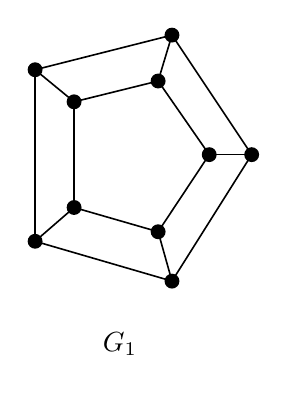
\begin{tikzpicture}[x=1cm,y=1cm,scale=1.1]
\coordinate (p0) at (0.600,3.120);
\coordinate (p1) at (1.520,1.740);
\coordinate (p2) at (0.600,0.280);
\coordinate (p3) at (-0.980,0.740);
\coordinate (p4) at (-0.980,2.720);
\coordinate (p5) at (0.440,2.590);
\coordinate (p6) at (1.030,1.740);
\coordinate (p7) at (0.440,0.850);
\coordinate (p8) at (-0.530,1.130);
\coordinate (p9) at (-0.530,2.350);
\draw[quizedge] (p0) -- (p1);
\draw[quizedge] (p0) -- (p4);
\draw[quizedge] (p0) -- (p5);
\draw[quizedge] (p1) -- (p2);
\draw[quizedge] (p1) -- (p6);
\draw[quizedge] (p2) -- (p3);
\draw[quizedge] (p2) -- (p7);
\draw[quizedge] (p3) -- (p4);
\draw[quizedge] (p3) -- (p8);
\draw[quizedge] (p4) -- (p9);
\draw[quizedge] (p5) -- (p6);
\draw[quizedge] (p5) -- (p9);
\draw[quizedge] (p6) -- (p7);
\draw[quizedge] (p7) -- (p8);
\draw[quizedge] (p8) -- (p9);
\node[quizvertex] at (p0) {};
\node[quizvertex] at (p1) {};
\node[quizvertex] at (p2) {};
\node[quizvertex] at (p3) {};
\node[quizvertex] at (p4) {};
\node[quizvertex] at (p5) {};
\node[quizvertex] at (p6) {};
\node[quizvertex] at (p7) {};
\node[quizvertex] at (p8) {};
\node[quizvertex] at (p9) {};
\node[font=\normalsize] at (0,-0.45) {$G_1$};
\end{tikzpicture}
\end{minipage}\hfill
\begin{minipage}{0.47\textwidth}\centering
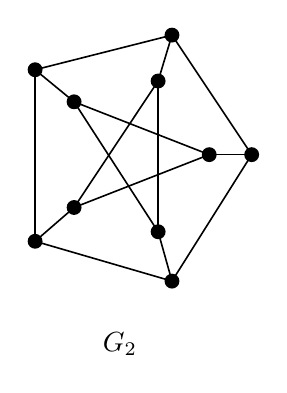
\begin{tikzpicture}[x=1cm,y=1cm,scale=1.1]
\coordinate (p0) at (0.600,3.120);
\coordinate (p1) at (1.520,1.740);
\coordinate (p2) at (0.600,0.280);
\coordinate (p3) at (-0.980,0.740);
\coordinate (p4) at (-0.980,2.720);
\coordinate (p5) at (0.440,2.590);
\coordinate (p6) at (1.030,1.740);
\coordinate (p7) at (0.440,0.850);
\coordinate (p8) at (-0.530,1.130);
\coordinate (p9) at (-0.530,2.350);
\draw[quizedge] (p0) -- (p1);
\draw[quizedge] (p0) -- (p4);
\draw[quizedge] (p0) -- (p5);
\draw[quizedge] (p1) -- (p2);
\draw[quizedge] (p1) -- (p6);
\draw[quizedge] (p2) -- (p3);
\draw[quizedge] (p2) -- (p7);
\draw[quizedge] (p3) -- (p4);
\draw[quizedge] (p3) -- (p8);
\draw[quizedge] (p4) -- (p9);
\draw[quizedge] (p5) -- (p7);
\draw[quizedge] (p5) -- (p8);
\draw[quizedge] (p6) -- (p8);
\draw[quizedge] (p6) -- (p9);
\draw[quizedge] (p7) -- (p9);
\node[quizvertex] at (p0) {};
\node[quizvertex] at (p1) {};
\node[quizvertex] at (p2) {};
\node[quizvertex] at (p3) {};
\node[quizvertex] at (p4) {};
\node[quizvertex] at (p5) {};
\node[quizvertex] at (p6) {};
\node[quizvertex] at (p7) {};
\node[quizvertex] at (p8) {};
\node[quizvertex] at (p9) {};
\node[font=\normalsize] at (0,-0.45) {$G_2$};
\end{tikzpicture}
\end{minipage}

\vspace{0.40cm}

\begin{minipage}{0.47\textwidth}\centering
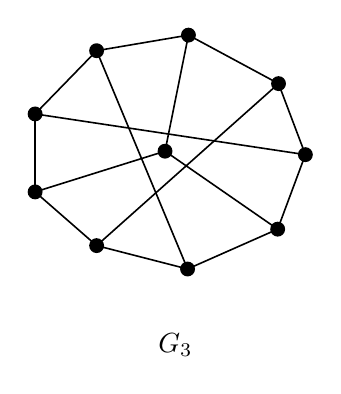
\begin{tikzpicture}[x=1cm,y=1cm,scale=1.1]
\coordinate (p0) at (0.150,3.130);
\coordinate (p1) at (1.190,2.570);
\coordinate (p2) at (1.500,1.750);
\coordinate (p3) at (1.180,0.890);
\coordinate (p4) at (0.140,0.430);
\coordinate (p5) at (-0.910,0.700);
\coordinate (p6) at (-1.620,1.320);
\coordinate (p7) at (-1.620,2.220);
\coordinate (p8) at (-0.910,2.950);
\coordinate (p9) at (-0.120,1.790);
\draw[quizedge] (p0) -- (p1);
\draw[quizedge] (p0) -- (p8);
\draw[quizedge] (p0) -- (p9);
\draw[quizedge] (p1) -- (p2);
\draw[quizedge] (p1) -- (p5);
\draw[quizedge] (p2) -- (p3);
\draw[quizedge] (p2) -- (p7);
\draw[quizedge] (p3) -- (p4);
\draw[quizedge] (p3) -- (p9);
\draw[quizedge] (p4) -- (p5);
\draw[quizedge] (p4) -- (p8);
\draw[quizedge] (p5) -- (p6);
\draw[quizedge] (p6) -- (p7);
\draw[quizedge] (p6) -- (p9);
\draw[quizedge] (p7) -- (p8);
\node[quizvertex] at (p0) {};
\node[quizvertex] at (p1) {};
\node[quizvertex] at (p2) {};
\node[quizvertex] at (p3) {};
\node[quizvertex] at (p4) {};
\node[quizvertex] at (p5) {};
\node[quizvertex] at (p6) {};
\node[quizvertex] at (p7) {};
\node[quizvertex] at (p8) {};
\node[quizvertex] at (p9) {};
\node[font=\normalsize] at (0,-0.45) {$G_3$};
\end{tikzpicture}
\end{minipage}\hfill
\begin{minipage}{0.47\textwidth}\centering
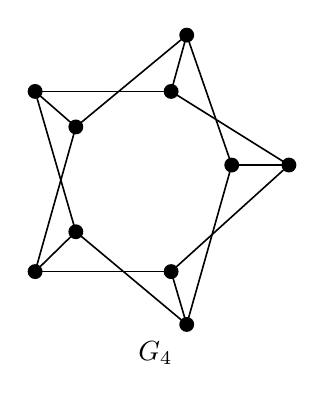
\begin{tikzpicture}[x=1cm,y=1cm,scale=1.1]
\coordinate (p0) at (-1.390,2.570);
\coordinate (p1) at (0.180,2.570);
\coordinate (p2) at (0.360,3.220);
\coordinate (p3) at (-0.920,2.160);
\coordinate (p4) at (0.880,1.720);
\coordinate (p5) at (1.540,1.720);
\coordinate (p6) at (-0.920,0.950);
\coordinate (p7) at (-1.390,0.490);
\coordinate (p8) at (0.180,0.490);
\coordinate (p9) at (0.360,-0.120);
\draw[quizedge] (p0) -- (p1);
\draw[quizedge] (p0) -- (p3);
\draw[quizedge] (p0) -- (p6);
\draw[quizedge] (p1) -- (p2);
\draw[quizedge] (p1) -- (p5);
\draw[quizedge] (p2) -- (p3);
\draw[quizedge] (p2) -- (p4);
\draw[quizedge] (p3) -- (p7);
\draw[quizedge] (p4) -- (p5);
\draw[quizedge] (p4) -- (p9);
\draw[quizedge] (p5) -- (p8);
\draw[quizedge] (p6) -- (p7);
\draw[quizedge] (p6) -- (p9);
\draw[quizedge] (p7) -- (p8);
\draw[quizedge] (p8) -- (p9);
\node[quizvertex] at (p0) {};
\node[quizvertex] at (p1) {};
\node[quizvertex] at (p2) {};
\node[quizvertex] at (p3) {};
\node[quizvertex] at (p4) {};
\node[quizvertex] at (p5) {};
\node[quizvertex] at (p6) {};
\node[quizvertex] at (p7) {};
\node[quizvertex] at (p8) {};
\node[quizvertex] at (p9) {};
\node[font=\normalsize] at (0,-0.45) {$G_4$};
\end{tikzpicture}
\end{minipage}
\end{center}
\end{problem}
\end{minipage}\par
\begin{solution}
Only $G_2\cong G_3$.

\par\medskip\noindent\textbf{Step 1.} We establish $G_2\cong G_3$ by constructing an explicit
isomorphism. Label the outer vertices of $G_2$ by $x_0, x_1, x_2, x_3, x_4$,
clockwise from the top, and its corresponding inner vertices by
$y_0, y_1, y_2, y_3, y_4$. In $G_3$, label the nine outer vertices by
$z_0, \dots, z_8$, clockwise from the top, and the central vertex by $z_9$.
The following bijection preserves all $15$ edges:
\[
\begin{array}{c|ccccc}
\text{Vertex}&x_0&x_1&x_2&x_3&x_4\\\hline
\text{Image}&z_0&z_1&z_2&z_3&z_9\\[3pt]
\text{Vertex}&y_0&y_1&y_2&y_3&y_4\\\hline
\text{Image}&z_8&z_5&z_7&z_4&z_6
\end{array}
\]
The outer $5$-cycle maps to $z_0z_1z_2z_3z_9z_0$. The five spokes map
to $z_0z_8$, $z_1z_5$, $z_2z_7$, $z_3z_4$, and $z_9z_6$; the inner edges
map to $z_8z_7$, $z_8z_4$, $z_5z_4$, $z_5z_6$, and $z_7z_6$.
These are exactly the edges of $G_3$, so $G_2\cong G_3$.

\par\medskip\noindent\textbf{Step 2.} We show that $G_1$ is isomorphic to neither $G_2$ nor
$G_3$. The graph $G_1$ contains a $4$-cycle through its top outer,
top inner, right inner, and rightmost outer vertices. The graph $G_2$
has no $4$-cycle: its two $5$-cycles are joined by a matching, so any
$4$-cycle would need two matching edges, one outer edge, and one inner
edge. This would require the same two indices to be adjacent in both
$5$-cycles, which is impossible: outer edges join consecutive indices,
while inner edges join indices differing by two. Since $G_2\cong G_3$ and
isomorphisms preserve cycle lengths, $G_1$ is isomorphic to neither.

\par\medskip\noindent\textbf{Step 3.} We show that $G_4$ is not isomorphic to any of the
other three graphs. It consists of a $10$-cycle together with five chords
joining vertices at distance $5$ along that cycle. Alternately coloring
the cycle's vertices gives a bipartition, and each chord also joins
opposite parts because $5$ is odd. Thus $G_4$ is bipartite. By contrast,
$G_1$, $G_2$, and $G_3$ each contain a $5$-cycle and hence are not
bipartite. Therefore $G_4$ is not isomorphic to any of them.
\end{solution}

\end{document}
